\section{Metody opisu klasycznej dynamiki cząstek}
W rozważaniach opuszczamy mechanikę Lagrangowską. 
\subsection{Mechanika newtonowska}
\textbf{Siła Lorenza}
\begin{equation}\label{sila_lorenza}
	\vec{F}_l \arg = q [ \vec{E} \arg+\vec{v}(t)\times\vec{B}\arg].
\end{equation}
Jeżeli postać siły jest określona, to równanie ruchu możemy 
zapisać w postaci
\begin{equation}
	m\frac{d^2\vec{r}(t)}{dt^2}=\vec{F}_L \arg  .
\end{equation}
Zauważmy, że w mechanice Newtonowskiej nie ma ograniczenia na 
postać siły $\vec{F}_L$.
\textbf{Przykład - równanie Langevine'a}
$$ m\frac{d^2}{dt^2} \vec{r}(t) = \vec{F}_R - \gamma\vec{v}(t) +
\vec{\Gamma}(t),$$
gdzie $\vec{F}_R$ to siła regularna (np. od zewnętrznego pola 
elektrycznego, $\gamma$ to współczynnik tarcia, a $\vec{\Gamma(t)}$ 
to siła stochastyczna.
Rozwiązując równania Newtona otrzymujemy różne $\vec{r}(t)$. 
Oznaczmy przez $\{ \vec{r}(t) \}$ - zbiór rozwiązań równania Newtona
$\equiv$ PRZESTRZEŃ KONFIGURACYJNA.

\begin{minipage}{0.5\textwidth}
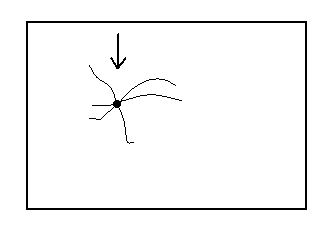
\includegraphics[width=\textwidth]{przestrzen_konfiguracyjna_newton.png}
\end{minipage}
\begin{minipage}{0.5\textwidth}
Wiele rozwiązań przechodzi \\
przez położenie początkowe \\
co powoduje \\ NIEJEDNOZNACZNOŚĆ \vspace{2.5cm}\\
\end{minipage}

$\left|\vec{r}(t)\right> $ - klasyczny stan cząstki w mechanice Newtona 
niewystarczający ze względu na brak determinizmu.

Stan cząstki opisany w spsób (trik dodający determinizm) $$\left| \vec{r}(t)
,\vec{v}(t) \right> \mbox{ - klasyczny stan cząstki}$$
$$
\begin{cases} 
	\dt \vec{r}(t)=\vec{v}(t) &\\
	m\dt \vec{v}(t)=\vec{F}(\vec{r},t)
\end{cases} + \mbox{war. początkowe (jednopunktowe)} 
\begin{cases}
	\vec{r}(t_0)=\vec{r}_0
	\vec{v}(t_0)=\vec{v}_0
\end{cases}
$$
\textbf{Uwaga}\\
Możemy określić $\vec{r}$ w chwili $t$, ale $\vec{v}$ okreśamy w otoczeniu $t$,
bo
$$\vec{v}_0 = \vec{v}(t_0) = \dt \vec{r}_{\Big|_{t=t_0}} = \lim_{\Delta t \to 0}
\frac{\vec{r}(t_0+\Delta t)-\vec{r}(t_0)}{\Delta t},$$
ewentualnie
$$\vec{v}_0 = \vec{v}(t_0) = \dt \vec{r}_{\Big|_{t=t_0}} = \lim_{\Delta t \to 0}
\frac{\vec{r}(t_0)-\vec{r}(t_0-\Delta t)}{\Delta t}.$$
\textbf{Wniosek}\\
Trikiem Tym uzyskujemy determinizm, z wyjątkiem infinitezymalnych zmian.

\subsection{Mechanika hamiltonowska}
W mechanice hamiltonowskiej nie używamy pojęcia siły, ale pojęcia potencjału,
co oznacza, że jest ona mniej ogólna.\\

\textbf{formalizm kanoniczny}\\
Funkcja Hamiltona: $ H\qpt$. Kosztem straty na ogólności, zyskujemy 
niezależność zmiennych uogólnionych $\vec{q}$ i $\vec{p}$.\\
$$ \left| \vec{q}(t), \vec{p}(t) \right> \mbox{ - klasyczny stan układu.} $$
Funkcja Hamiltona przybiera wartość całkowitej energii mechanicznej układu, jeżeli
siły sziałające na układ są potencjalne, a potencjał nie zależy od czasu.
$$ H\qp = \underbrace{J(\vec{q},\dot{\vec{q}}(\vec{q},\vec{p}))}_{\mbox{
część kinetyczna}} + \underbrace{U(\vec{q})}_{\mbox{część potencjalna}}.$$
$q,p$ - współrzędne i pędy uogólnione, zgodne z więzami skleronomicznymi, czyli takimi, że nie zależą jawnie od czasu.
\subsubsection{Przestrzeń fazowa $\mu$}
\textbf{Definicja}\\
Przestrzenią fazowa $\mu$ układu mechanicznego nazywamy parzysto-wymiarową 
przestrzeń symplektyczną, której elementami są punkty fazowe o współrzędnych 
$\qp$, które reprezentują stany klasyczne układu.
$$ H\qpt = J(\vec{q},\dot{\vec{q}}\qp)+U\qpt $$
$$ H:\mu \times \mathbb{R} \to \mathbb{R}, \quad \mbox{kl. } C^1[\mu]. $$
\textbf{Przykład}\\
$$ \vec{F}_L \arg = q[\E+\v (t)\times\B]$$
$$ \phi (\vec{r},\vec{v},t) = q[ \underbrace{V\arg}_{\mbox{pot. skalarny}}
-\v (t) \cdot \underbrace{\vec{A} \arg }_{\mbox{pot. wektorowy}}]. $$
Poprzez transformatę Legendre'a
$$H(\vec{r},\vec{p}) = \underbrace{\frac{1}{2m} [\vec{p}+q\vec{A}\arg ]^2}_{\mbox{
część kinetyczna}} + \underbrace{U\arg}_{\mbox{część potencjalna}}.$$
\subsubsection{Funkcja Hamiltona w przybliżeniu minimalnego sprzężenia 
eletromagnetycznego}
$$H(\vec{r},\vec{p}) = \frac{1}{2m} [\vec{p}+q\vec{A}\arg ]\cdot[\vec{p}+
q\vec{A}\arg ] + U\arg= \frac{p^2}{2m} + U\arg + \frac{q}{m}\vec{p}\cdot\vec{A}\arg
+\frac{q^2}{2m}A^2\arg \approx$$
$$\approx \big| \mbox{linearyzacja, zakładając, że A jest małe} \big| \approx
\underbrace{\frac{p^2}{2m} + U\arg}_{H_0\rpt} + \frac{q}{m} \vec{p} \cdot \vec{A}
\arg,$$
gdzie $H_0\rpt$ to niezaburzona funkcja Hamiltona, a pozostały składnik jest 
zaburzeniem liniowym spowodowanym potencjałem wektorowym $\vec{A}$.
\subsubsection{Kanoniczne równania Hamiltona}
\begin{equation}
\begin{cases}
	\dot{\vec{q}} (t) = \nab{p} H\qpt \\
	\dot{\vec{p}} (t) = - \nab{q} H\qpt 
\end{cases} +
\begin{cases}
	\vec{q}(t_0) = \vec{q}_0 \\
	\vec{p}(t_0) = \vec{p}_0
\end{cases}
\end{equation}
$$\begin{cases} 
	\vec{q}(t) = \vec{q}(t_0) + \int_{t_0}^t dt' \nab{p} H(\vec{q},\vec{p},t') \\
	\vec{p}(t) = \vec{p}(t_0) + \int_{t_0}^t dt' \nab{q} H(\vec{q},\vec{p},t').
\end{cases}$$
Rozwiazanie powyższe wyznacza trajektorię fazową w przestrzni fazowej, 
która to jest zbiorem klasycznych stanów realizowanych przez układ 
w kolejnych chwilach czasu $t$.\\
\textbf{Inna forma równań Hamiltona}\\
Wprowadzamy wektor fazowy $ \vec{w}\qp $ oraz hamiltonowskie pole wektorowe
$\vec{X}_H \qpt$. Wtedy
\begin{equation} \dt \vec{w}\qp = \vec{X}_H \qpt \end{equation}
\begin{equation} \dt 
\left[ \begin{matrix} \vec{q}(t) \\ \vec{p}(t)  \end{matrix} \right] 
= \underbrace{\left[ \begin{matrix} 0 & 1 \\ -1 & 0  \end{matrix} \right]}_{g}
\left[ \begin{matrix} \nab{q}H\qpt \\ \nab{p}H\qpt \end{matrix} \right]
,\end{equation}
gdzie $g$ to anysymetryczny tensor metryczny, który określa geomerię symplektyczną
przestreni fazowej.
\subsubsection{Zależność funkcji Hamitona od czasu}
$H\qpt$ może się zmieniać w czasie na dwa sposoby
\begin{enumerate}
	\item $\vec{q} = \vec{q}(t),\ \vec{p} = \vec{p}(t),$
	\item $t$ (jawnie)
\end{enumerate}
$$\dt H\qpt =\left[ \dt \vec{q}(t) \right]\cdot \nab{q} H\qpt +
\left[ \dt \vec{p}(t)\right] \cdot \nab{p} H\qpt + \partial_t H\qpt =
$$
$$=\nab{p}H\qpt \cdot \nab{q}H\qpt - \nab{q}H\qpt \cdot \nab{p}H\qpt + \partial_t
H\qpt.$$
Zatem
$$\dt H\qpt = \partial_t H\qpt.$$
Stąd wynika, iż funkcja Hamiltona zmieniasię tak w czasie jak zależy od czasu.\\
Jeżeli $H=H\qp$ to $\dt H\qp = 0$. Stąd wynika, że energia jest zachowana 
wzdłuż trajektorii fazowej.
\subsection{Nawiasy Poissona}
\textbf{definicja}\\
$f\qpt $, $g\qpt$ - funkcje klasy $C^1[\mu]$. Wtedy definiujemy 
$$ \{ f,g \}= \nab{q} f\qpt \cdot \nab{p} g\qpt - \nab{p} f\qpt \cdot \nab{q}
g\qpt = \left[ \begin{matrix} \nab{q} f\qpt & \nab{p}f\qpt  \end{matrix} \right]
 \left[ \begin{matrix} 0 & 1 \\ -1 & 0 \end{matrix} \right] 
 \left[ \begin{matrix} \nab{q} g\qpt \\ \nab{p} g\qpt \end{matrix} \right].$$
\textbf{Pożytki:}
\begin{enumerate}
	\item łatwiej znaleźć niektóre całki ruchu $C\qp : \{ C\qp, H\qp \} =0$.
	\item równania Hamiltona można zapisać następująco
	\begin{equation}
		\begin{cases}
		\dt \vec{q} =  \{ \vec{q} , H\qpt \} \\
		\dt \vec{p} =  \{ \vec{p} , H\qpt \} 
		\end{cases}
	\end{equation}
\end{enumerate}
\textbf{Przykłady}
\begin{enumerate}
	\item Niech $H\qp = \frac{p^2}{2m} + U(\vec{q})$
	$$ \vec{v} (t) = \{ \vec{q} , \frac{p^2}{2m} + U(\vec{q}) \} = \{ \vec{q}
	, \frac{p^2}{2m} \} + \overbrace{\{ \vec{q} , U(\vec{q}) \}}^{=0} = 
	\nab{q}\vec{q} \cdot \nab{p} \frac{p^2}{2m} - \nab{p} \vec{q} \cdot 
	\nab{q} \frac{p^2}{2m} = \frac{\vec{p}}{m}$$
	$$\implies \vec{p}(t) = m \vec{v}(t).$$
	\item Niech $H\qp = \frac{p^2}{2m} + U(\vec{q},\vec{p})$
	$$ \vec{v}(t) = \{ \vec{q}, H\qp \} = \ldots = \frac{1}{m} \vec{p}(t)
	+\nab{p} U\qp \implies \vec{p} (t) = m\vec{v}(t) - m\nab{p}U\qp$$
	\item Rozważmy zaburzenie $H'\arg = \frac{q}{m} \vec{p}\cdot \vec{A}\arg=$
	$$= q\vec{v} \cdot \vec{A}\arg = q \int d^3r'\delta(\vec{r}\ ' - 
	\vec{r}(t)) \vec{v}(t)\cdot \vec{A} (\vec{r}\ ',t)=\int d^3r' \underbrace{
	q \delta(\vec{r}\ ' - \vec{r}(t))}_{\rho (\vec{r}\ ',t)} \vec{v}(t)\cdot 
	\vec{A}(\vec{r}\ '	, t ) =$$
	$$= \int d^3r' \underbrace{\rho (\vec{r}\ ',t) \vec{v}(t)}_{\vec{j}
	(\vec{r}\ ',t)} \cdot \vec{A}(\vec{r}\	 ' ,t) = \int d^3r \vec{j} 
	(\vec{r}\ ',t)\cdot \vec{A} (\vec{r}\ ' ,t).$$
	Przedstawiliśmy zaburzenia za pomocą pola elektrycznego.
\end{enumerate}

